
%使用XeLaTeX编译
%版权所有,翻版必究
%本文件由程序自动生成,任何修改将被覆盖
%2019 年 01 月 23 日




\FloatBarrier
\section{
曲线图导引
}\label{c000017s01}


曲线图(Qt Charts)模块默认并不被安装,
但是它非常有用,
读者应当总是安装这个模块。

要使用Qt Charts模块需要在QML头添加:\begin{littlelongworld}
import QtCharts 2.3
\end{littlelongworld}
并在工程文件添加:\begin{littlelongworld}
QT {\sourcefonttwo{}+}{\sourcefonttwo{}=} charts
\end{littlelongworld}
\hspace*{\parindent}\filesourcenumbernameone\ \ref{f000080}展示
了一个简单的Qt Charts模块的应用。

%../chapter08/firstchart/the_book.png
%begin图片
\begin{figure}[htb] %浮动体 here and top ...
%there must use marginnote ...
\marginnote{\setlength\fboxsep{2pt}\fbox{\footnotesize{\kaishu\figurename\,}\footnotesize{\ref{p000049}}}}\centering %中心对齐
\setlength\fboxsep{0pt}\fcolorbox[rgb]{0,0,0}{0.97,0.98,0.99}{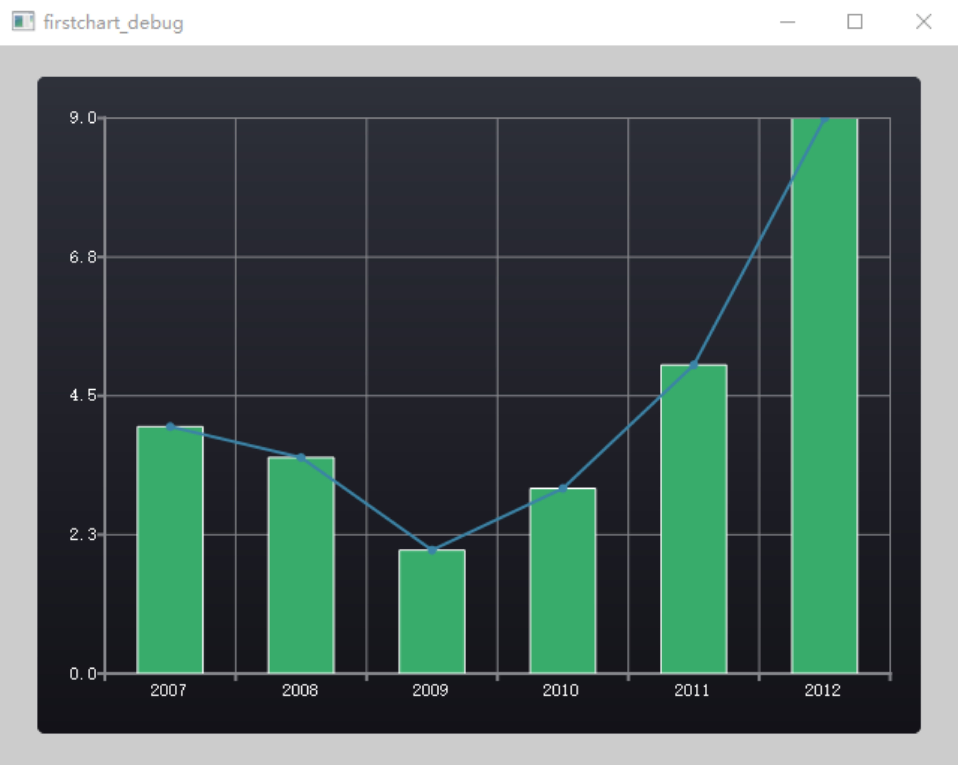
\includegraphics[width=0.95\textwidth]{the_book_image/p000049.pdf}} %图片路径
\caption{QtCharts} %标题
\label{p000049} %索引
\end{figure}
%end图片


%../chapter08/firstchart/myqml/firstchart/main.qml
%\begin{spacing}{1.0}
\refstepcounter{filesourcenumber}\label{f000080}    %增加源代码编号
\FloatBarrier                                  %强制完成浮动体布局
\begin{thebookfilesourceone}[escapeinside={(*@}{@*)},
caption=GoodLuck,
title=\filesourcenumbernameone \thefilesourcenumber
]
/*firstchart/main.qml*/
import QtQuick 2.9
import QtCharts 2.3

Rectangle {

    id : idRoot
    width: 640;
    height: 480;
    color: Qt.rgba(0.8,0.8,0.8,1);

    ChartView{
        anchors.centerIn: parent ;
        width: parent.width * 0.95 ;
        height: parent.height * 0.95 ;
        theme: ChartView.ChartThemeDark
        antialiasing: true
        dropShadowEnabled : true
        legend.visible : false
        animationOptions :ChartView.AllAnimations

        BarSeries {
            id: idBar
            axisX: BarCategoryAxis {
                categories: [
                    "2007",
                    "2008",
                    "2009",
                    "2010",
                    "2011",
                    "2012" ] }
            BarSet {
                label: qsTr( "FirstChart" );
                values: [4, 3.5, 2, 3, 5, 9]
            }
        }

        LineSeries{
            XYPoint { x: 0; y: 4 }
            XYPoint { x: 1; y: 3.5 }
            XYPoint { x: 2; y: 2 }
            XYPoint { x: 3; y: 3 }
            XYPoint { x: 4; y: 5 }
            XYPoint { x: 5; y: 9 }
            axisX: idBar.axisX
            axisY: idBar.axisY
            pointsVisible: true
            pointLabelsVisible : false
        }

    }

}/*~Rectangle*/(*@\marginpar[\hfill\setlength\fboxsep{2pt}\fbox{\footnotesize{\kaishu\parbox{1em}{\setlength{\baselineskip}{2pt}\filesourcenumbernameone}}\footnotesize{\thefilesourcenumber}}]{\setlength\fboxsep{2pt}\fbox{\footnotesize{\kaishu\parbox{1em}{\setlength{\baselineskip}{2pt}\filesourcenumbernameone}}\footnotesize{\thefilesourcenumber}}}@*)\end{thebookfilesourceone}          %抄录环境
\addtocounter{lstlisting}{-1}   %sub lstlisting counter ...
%\end{spacing}


\begin{comment}
介绍代码..........................
\end{comment}

如\filesourcenumbernameone\ \ref{f000080}所
示:
\begin{itemize}
\item 第12行使用ChartView作为
Qt Charts各类曲线的
视图。
    \begin{itemize}
\item 第16行定义了ChartView的主题。
\item 第19行要求隐藏
图例。
\item 第20行启用所有动画。
    \end{itemize}
\item 第22行、第38行
分别定义了柱状图和折线图。
\item 第45\raisebox{0.16ex}{\sourcefonttwo\~{}}46行
规定折线图使用柱状图的坐标系。

\end{itemize}

视图、
曲线、
坐标轴、
图例、
动画
与
主题。
这些是Qt Charts支持良好的部分。

除此之外,Qt Charts也支持
输入设备(比如鼠标键盘)响应和
移动视图。

有时候需要给Qt Charts增加一些额外自定义元素,
那么就不得不深入Qt Charts源码并多费心思。
毕竟Qt Charts是为QGraphicsView而设计的,
对于Qt Quick而言,Qt Charts的
一些设计就过于呆板。


% ______all_key_words
% the_book_chapter the_book_subsection the_book_subsubsection
% the_book_section the_book_image the_book_table
% the_book_file the_book_tree_file the_book_command_file
% littlelongworld tabbing ref
% figurename tablename filesourcenumbernameone
% treeindexnumbernameone commandnumbernameone footnote
% item itemize comment textbullet
% \hspace*{\parindent}







%使用XeLaTeX编译
%版权所有,翻版必究
%本文件由程序自动生成,任何修改将被覆盖
%2019 年 01 月 23 日



